%%%%%%%%%%%%%%%%%%%%%%%%%%%%%%%%%%%%%%%%%%%%%%%%%%%%%%%%%%%%%%%%%%%%%%%%
% Beamer Presentation - LaTeX - Template Version 1.0 (10/11/12)
% This template has been downloaded from: http://www.LaTeXTemplates.com
% License: % CC BY-NC-SA 3.0 (http://creativecommons.org/)
% Modified by Rahmat M. Samik-Ibrahim

% REV420: Sat 24 Aug 2024 08:00
% REV417: Sun 28 Jan 2024 16:00
% REV403: Thu 23 Feb 2023 08:00
% REV371: Mon 28 Feb 2022 10:00
% REV363: Mon 20 Dec 2021 15:00
% STARTX: Wed 14 Sep 2016 10:00
%%%%%%%%%%%%%%%%%%%%%%%%%%%%%%%%%%%%%%%%%%%%%%%%%%%%%%%%%%%%%%%%%%%%%%%%%

% PACKAGES AND THEMES 
\documentclass[aspectratio=169, xcolor=table, notheorems, hyperref={pdfpagelabels=false}]{beamer}
%%%%%%%%%%%%%%%%%%%%%%%%%%%%%%%%%%%%%%%%%%%%%%%%%%%%%%%%%%%%%%%%%%%%%%%%
% Beamer Presentation - LaTeX - Template Version 1.0 (10/11/12)
% This template has been downloaded from: http://www.LaTeXTemplates.com
% License: % CC BY-NC-SA 3.0 (http://creativecommons.org/)
% Modified by Rahmat M. Samik-Ibrahim
% REV419: Wed 24 Jul 2024 17:00
% REV383: Tue 12 Jul 2022 10:00
% REV316: Wed 14 Jul 2021 13:00
% REV198: Wed 13 Mar 2019 16:00
% REV005: Mon  2 Oct 2017 14:00
% STARTX: Thu 25 Aug 2016 14:00
%%%%%%%%%%%%%%%%%%%%%%%%%%%%%%%%%%%%%%%%%%%%%%%%%%%%%%%%%%%%%%%%%%%%%%%%%

%% ZCZC NNNN
\newtheorem{example}{Example}

%%%%%%%%%%%%%%%%%%%%%%%%%%%%%%%%%%%%%%%%%%%%%%%%%%%%%%%%%%%%%%%%%%%%%%%%%

\let\Tiny=\tiny
\mode<presentation> {
% The Beamer class comes with a number of default slide themes
% which change the colors and layouts of slides. Below this is a list
% of all the themes, uncomment each in turn to see what they look like.
%\usetheme{Boadilla}
\usetheme{Madrid}
% ZCZC %%%%%%%%%%%%%%%%%%%%%%%%%%%%%%%%%%%%%%%%%%%%%%%%%%%%%%%%%%%%%%%%%%
% \usetheme{default} \usetheme{AnnArbor} \usetheme{Antibes} \usetheme{Bergen}
% \usetheme{Berkeley} \usetheme{Berlin} \usetheme{CambridgeUS} 
% \usetheme{Copenhagen} \usetheme{Darmstadt} \usetheme{Dresden}
% \usetheme{Frankfurt} \usetheme{Goettingen} \usetheme{Hannover}
% \usetheme{Ilmenau} \usetheme{JuanLesPins} \usetheme{Luebeck}
% \usetheme{Malmoe} \usetheme{Marburg} \usetheme{Montpellier}
% \usetheme{PaloAlto} \usetheme{Pittsburgh} \usetheme{Rochester}
% \usetheme{Singapore} \usetheme{Szeged} \usetheme{Warsaw}
% NNNN %%%%%%%%%%%%%%%%%%%%%%%%%%%%%%%%%%%%%%%%%%%%%%%%%%%%%%%%%%%%%%%%%%
% As well as themes, the Beamer class has a number of color themes
% for any slide theme. Uncomment each of these in turn to see how it
% changes the colors of your current slide theme.
%\usecolortheme{orchid}
%\usecolortheme{rose}
%\usecolortheme{seagull}
%\usecolortheme{seahorse}
\usecolortheme{whale}
% ZCZC %%%%%%%%%%%%%%%%%%%%%%%%%%%%%%%%%%%%%%%%%%%%%%%%%%%%%%%%%%%%%%%%%%
%\usecolortheme{albatross} \usecolortheme{beaver} \usecolortheme{beetle}
%\usecolortheme{crane} \usecolortheme{dolphin} \usecolortheme{dove}
%\usecolortheme{fly} \usecolortheme{lily} \usecolortheme{wolverine}
% NNNN %%%%%%%%%%%%%%%%%%%%%%%%%%%%%%%%%%%%%%%%%%%%%%%%%%%%%%%%%%%%%%%%%%
% To remove the footer line in all slides uncomment this line
%\setbeamertemplate{footline} 
% To replace the footer line in all slides uncomment this line
%\setbeamertemplate{footline}[page number] 
% To remove the navigation symbols from the bottom uncomment this line
\setbeamertemplate{navigation symbols}{} 
}

\usepackage{array}       % ZCZC
\usepackage{amssymb}     % ZCZC
\usepackage{bold-extra}  % ZCZC
\usepackage{booktabs}    % Allows \toprule, \midrule and \bottomrule in tables
\usepackage{caption}
\usepackage[T1]{fontenc} % ZCZC << >>
\usepackage{graphicx}    % Allows including images
\usepackage{listings}    % listing
\usepackage{lmodern}     % ZCZC
\usepackage{perpage}     % reset footnote per page
\usepackage{geometry}    % ZCZC
\usepackage{adjustbox}   % ZCZC
\usepackage{multicol}    % ZCZC
\usepackage{multirow}    % ZCZC
\usepackage{pgf-pie}     % ZCZC pie chart

% \definecolor{links}{HTML}{2A1B81}
\definecolor{links}{HTML}{0011FF}
\hypersetup{colorlinks,linkcolor=,urlcolor=links}

% \usepackage{xcolor}
% \usepackage[colorlinks = true,
%             linkcolor = blue,
%             urlcolor  = blue,
%             citecolor = blue,
%             anchorcolor = blue]{hyperref}

\captionsetup[table]{name=Tabel}
\makeatletter
\def\input@path{{src/}}
\makeatother
\graphicspath{{src/}}      % src directory
\MakePerPage{footnote}     % reset page

% NNNN %%%%%%%%%%%%%%%%%%%%%%%%%%%%%%%%%%%%%%%%%%%%%%%%%%%%%%%%%%%%%%%%%%

%% % XXXXXXXXXXXXXXXXXXXXXXXXXXXXXXXXXXXXXXXXXXXXXXXXXXXXXXXXXXXXXXXXXXXXXXXXXX
%% % The short title appears at the bottom of every slide, 
%% % the full title is only on the title page
%% \title[Judul Pendek]{Judul Panjang dan Lengkap} 
%% \author{Cecak bin Kadal}
%% \institute[UILA]
%% {
%% University of Indonesia at Lenteng Agung \\ 
%% \medskip
%% \textit{cecak@binKadal.com}
%% }
%% \date{REV00 24-Aug-2016}
%% % \date{\today}
%% 

%% % XXXXXXXXXXXXXXXXXXXXXXXXXXXXXXXXXXXXXXXXXXXXXXXXXXXXXXXXXXXXXXXXXXXXXXXXXX
%% \begin{document}
%% \section{Judul}
%% \begin{frame}
%% \titlepage
%% \end{frame}
%% 
%% % XXXXXXXXXXXXXXXXXXXXXXXXXXXXXXXXXXXXXXXXXXXXXXXXXXXXXXXXXXXXXXXXXXXXXXXXXX
%% \section{Agenda}
%% \begin{frame}
%% \frametitle{Agenda}
%% % Throughout your presentation, if you choose to use \section{} and 
%% % \subsection{} commands, these will automatically be printed on 
%% % this slide as an overview of your presentation
%% \tableofcontents 
%% \end{frame}
%% 
%% % XXXXXXXXXXXXXXXXXXXXXXXXXXXXXXXXXXXXXXXXXXXXXXXXXXXXXXXXXXXXXXXXXXXXXXXXXX
%% \section{UUD dan Pancasila}
%% \subsection{UUD}
%% \begin{frame}
%% \frametitle{Pembukaan}
%% Bahwa sesungguhnya kemerdekaan itu ialah hak segala bangsa dan oleh 
%% sebab itu, maka penjajahan diatas dunia harus dihapuskan karena 
%% tidak sesuai dengan perikemanusiaan dan perikeadilan.
%% \\~\\
%% Atas berkat rahmat Allah Yang Maha Kuasa dan dengan didorongkan oleh 
%% keinginan luhur, supaya berkehidupan kebangsaan yang bebas, maka 
%% rakyat Indonesia menyatakan dengan ini kemerdekaannya.
%% \end{frame}
%% 
%% % XXXXXXXXXXXXXXXXXXXXXXXXXXXXXXXXXXXXXXXXXXXXXXXXXXXXXXXXXXXXXXXXXXXXXXXXXX
%% \begin{frame}
%% \frametitle{Alenia Ketiga}
%% Kemudian daripada itu untuk membentuk suatu pemerintah negara Indonesia 
%% yang melindungi segenap bangsa Indonesia dan seluruh tumpah darah Indonesia 
%% dan untuk memajukan kesejahteraan umum, mencerdaskan kehidupan bangsa, dan 
%% ikut melaksanakan ketertiban dunia yang berdasarkan kemerdekaan, perdamaian 
%% abadi dan keadilan sosial, maka disusunlah kemerdekaan kebangsaan Indonesia 
%% itu dalam suatu Undang-Undang Dasar negara Indonesia, yang terbentuk dalam 
%% suatu susunan negara Republik Indonesia yang berkedaulatan rakyat dengan 
%% berdasar kepada:
%% \begin{itemize}
%% \item Ketuhanan Yang Maha Esa,
%% \item kemanusiaan yang adil dan beradab,
%% \item persatuan Indonesia,
%% \item dan kerakyatan yang dipimpin oleh hikmat kebijaksanaan 
%%       dalam permusyawaratan/ perwakilan,
%% \item serta dengan mewujudkan suatu keadilan sosial bagi seluruh rakyat 
%%       Indonesia.
%% \end{itemize}
%% \end{frame}
%% 
%% % XXXXXXXXXXXXXXXXXXXXXXXXXXXXXXXXXXXXXXXXXXXXXXXXXXXXXXXXXXXXXXXXXXXXXXXXXX
%% \subsection{Pancasila}
%% \begin{frame}
%% \frametitle{Tujuh Kunci Pokok}
%% \begin{block}{Pertama - Kedua - Ketiga}
%% Indonesia ialah negara berdasarkan hukum.
%% Sistem konstitusional.
%% Kekuasaan negara tertinggi di tangan MPR.
%% \end{block}
%% 
%% \begin{block}{Keempat - Kelima}
%% Presiden adalah penyelenggara pemerintahan tertinggi di bawah MPR.
%% Adanya pengawasan DPR.
%% \end{block}
%% 
%% \begin{block}{Keenam}
%% Menteri negara adalah pembantu presiden dan tidak bertanggung jawab 
%% kepada DPR.
%% \end{block}
%% 
%% \begin{block}{Ketujuh}
%% Kekuasaan kepala negara tidak tak tebatas.
%% \end{block}
%% 
%% \end{frame}
%% 
%% % XXXXXXXXXXXXXXXXXXXXXXXXXXXXXXXXXXXXXXXXXXXXXXXXXXXXXXXXXXXXXXXXXXXXXXXXXX
%% \section{Rupa-rupa}
%% \subsection{Kolom}
%% \begin{frame}
%% \frametitle{Kolom}
%% % The "c" option specifies centered vertical alignment 
%% % while the "t" option is used for top vertical alignment
%% \begin{columns}[c] 
%% % Left column and width
%% \column{.45\textwidth} 
%% \textbf{Heading}
%% \begin{enumerate}
%% \item Satu-satu
%% \item Dua-dua
%% \item Tiga-tiga
%% \item Satu-dua-tiga
%% \end{enumerate}
%% 
%% % Right column and width
%% \column{.5\textwidth}
%% Satu-satu~\dots{} aku sayang ibu!
%% Dua-dua~\ldots{} juga sayang ayah!
%% Tiga-tiga~\ldots{} sayang adik kakak!
%% Satu-dua-tiga~\ldots{} sayang semuanya!
%% 
%% \end{columns}
%% \end{frame}
%% 
%% % XXXXXXXXXXXXXXXXXXXXXXXXXXXXXXXXXXXXXXXXXXXXXXXXXXXXXXXXXXXXXXXXXXXXXXXXXX
%% \subsection{Tabel}
%% \begin{frame}
%% \frametitle{Tabel}
%% \begin{table}
%% \begin{tabular}{l l l}
%% \toprule
%% \textbf{Nama} & \textbf{NPM} & \textbf{Tanggal Lahir}\\
%% \midrule
%% Cecak bin Kadal & 1234567890 & 1 Jan 2015 \\
%% Aneh bin Ajaib  & 0987654321 & 31 Des 2014 \\
%% \bottomrule
%% \end{tabular}
%% \caption{Keterangan Tabel}
%% \end{table}
%% \end{frame}
%% 
%% % XXXXXXXXXXXXXXXXXXXXXXXXXXXXXXXXXXXXXXXXXXXXXXXXXXXXXXXXXXXXXXXXXXXXXXXXXX
%% \subsection{Teori}
%% \begin{frame}
%% \frametitle{Teori}
%% \begin{theorem}[Teori Satu Batu]
%% $E = mc^2$
%% \end{theorem}
%% \end{frame}
%% 
%% % XXXXXXXXXXXXXXXXXXXXXXXXXXXXXXXXXXXXXXXXXXXXXXXXXXXXXXXXXXXXXXXXXXXXXXXXXX
%% \subsection{Verbatim}
%% % Need to use the fragile option when verbatim is used in the slide
%% \begin{frame}[fragile] 
%% \frametitle{Verbatim}
%% \begin{example}[Teori Satu Batu]
%% \begin{verbatim}
%% \begin{theorem}[Teori Satu Batu]
%% $E = mc^2$
%% \end{theorem}
%% \end{verbatim}
%% \end{example}
%% \end{frame}
%% 
%% % XXXXXXXXXXXXXXXXXXXXXXXXXXXXXXXXXXXXXXXXXXXXXXXXXXXXXXXXXXXXXXXXXXXXXXXXXX
%% \subsection{Gambar}
%% \begin{frame}
%% \frametitle{Gambar}
%% \begin{figure}
%% \includegraphics[width=0.5\linewidth]{2}
%% \caption{Ini Gambar JPG}
%% \end{figure}
%% \end{frame}
%% 
%% % XXXXXXXXXXXXXXXXXXXXXXXXXXXXXXXXXXXXXXXXXXXXXXXXXXXXXXXXXXXXXXXXXXXXXXXXXX
%% \subsection{Rujukan}
%% % Need to use the fragile option when verbatim is used in the slide
%% \begin{frame}[fragile] 
%% \frametitle{Rujukan dan Kutipan}
%% Contoh penggunaan \verb|\cite| ketika mengutip\cite{p1}.
%% Perhatian: Beamer tidak mengerti \verb|\BibTeX|~\ldots
%% \footnotesize{
%%   \begin{thebibliography}{99} 
%%   \bibitem[Smith, 2012]{p1} John Smith (2012)
%%      \newblock Katak dalam Tempurung
%%      \newblock \emph{Jurnal Kelapa dan Amfibi} 12(3), 45 -- 678.
%%   \end{thebibliography}
%% }
%% \end{frame}
%% 
%% % XXXXXXXXXXXXXXXXXXXXXXXXXXXXXXXXXXXXXXXXXXXXXXXXXXXXXXXXXXXXXXXXXXXXXXXXXX
%% \subsection{Selesai}
%% \begin{frame}
%% \Huge{\centerline{Selesai}}
%% \end{frame}
%% 
%% % XXXXXXXXXXXXXXXXXXXXXXXXXXXXXXXXXXXXXXXXXXXXXXXXXXXXXXXXXXXXXXXXXXXXXXXXXX
%% \end{document}

\newcommand{\revision}{%
REV426: Wed 13 Nov 2024 04:00
}
% w! tmptmp
% REV426: Wed 13 Nov 2024 04:00
% REV419: Wed 24 Jul 2024 17:00
% REV409: Tue 08 Aug 2023 12:00
% REV399: Fri 03 Feb 2023 20:00
% REV339: Sat 04 Sep 2021 12:00
% STARTS: Wed 24 Aug 2016 19:00
%%%%%%%%%%%%%%%%%%%%%%%%%%%%%%%%%%%%%
\newcommand{\kopikopi}{\textcopyright{}2016-2024 CBKadal + VauLSMorg}



% XXXXXXXXXXXXXXXXXXXXXXXXXXXXXXXXXXXXXXXXXXXXXXXXXXXXXXXXXXXXXXXXXXXXXXXXXX
% The short title appears at the bottom of every slide, 
% the full title is only on the title page
% \date{\today}
\title[\kopikopi]
{CSGE602055 Operating Systems \\ 
CSF2600505 Sistem Operasi \\
Week 09:
Storage, Firmware, Bootloader, \& Systemd}
\author{C. BinKadal}
\institute[SdnBhd]
{
Sendirian Berhad\\
\medskip
\url{https://docos.vlsm.org/Slides/os09.pdf}
\\ \texttt{Always check for the latest revision!}
}
\date{\revision}

% XXXXXXXXXXXXXXXXXXXXXXXXXXXXXXXXXXXXXXXXXXXXXXXXXXXXXXXXXXXXXXXXXXXXXXXXXX
\begin{document}

\lstset{
basicstyle=\ttfamily\tiny, % \tiny \small \footnotesize 
breakatwhitespace=true,
language=C,
columns=fullflexible,
keepspaces=true,
breaklines=true,
tabsize=3, 
showstringspaces=false,
extendedchars=true}

\section{Start}
\begin{frame}
\titlepage
\end{frame}

% XXXXXXXXXXXXXXXXXXXXXXXXXXXXXXXXXXXXXXXXXXXXXXXXXXXXXXXXXXXXXXXXXXXXXXXXXX

%%%%%%%%%%%%%%%%%%%%%%%%%%%%%%%%%%%%%%%%%%%%%%%%%%%%%%%%%%%%%%%%%%%%%%%%%
% REV418: Tue 30 Jan 2024 22:00
% REV406: Sat 05 Aug 2023 14:00
% REV399: Thu 02 Feb 2023 00:00
% REV369: Mon 14 Feb 2022 09:00
% REV328: Sat 14 Aug 2021 06:00
% STARTX: Wed 14 Sep 2016 10:00
%%%%%%%%%%%%%%%%%%%%%%%%%%%%%%%%%%%%%%%%%%%%%%%%%%%%%%%%%%%%%%%%%%%%%%%%%

\begin{frame}[fragile]
\section{OS241 Schedule}
\frametitle{OS241\footnote{%
) This information will be on \textbf{EVERY} page two (2) of this course material.}): 
Operating Systems Schedule 2023 - 2}

\vspace{5pt}

\scalebox{0.99}{%
\begin{tabular}{|c|c|l|l|}
\hline
\textbf{Week} & 
\textbf{Topic}\footnote{%
) For schedule, see \url{https://os.vlsm.org/\#idx02}}) & \textbf{OSC10}\footnote{%
    ) Silberschatz et. al.: \textbf{Operating System Concepts}, $10^{th}$ Edition, 2018.}) \\
\hline
Week 00  & Overview (1), Assignment of Week 00           & Ch. 1, 2      \\
Week 01  & Overview (2), Virtualization \& Scripting     & Ch. 1, 2, 18. \\
Week 02  & Security, Protection, Privacy, \& C-language. & Ch. 16, 17.   \\
Week 03  & File System \& FUSE  & Ch. 13, 14, 15.                        \\
Week 04  & Addressing, Shared Lib, \& Pointer & Ch. 9. \\
Week 05  & Virtual Memory & Ch. 10. \\
\hline
Week 06  & Concurrency: Processes \& Threads & Ch. 3, 4. \\
Week 07  & Synchronization \& Deadlock & Ch. 6, 7, 8. \\
Week 08  & Scheduling + W06/W07 & Ch. 5. \\
Week 09  & Storage, Firmware, Bootloader, \& Systemd & Ch. 11. \\
Week 10  & I/O \& Programming & Ch. 12. \\%
% MidTerm  & 00 XXX 2020 (XX:XX-XX:XX) & MidTerm (UTS) & \cellcolor{red!44} TBA! \\
% Reserved & 00 XXX - 00 XXX 2020 & Q \& A & \\
% Final    & 00 XXX 2020 XX:XX & First Part Final  (UAS tahap I)  & \cellcolor{red!44} This schedule is   \\
% Extra    & NA & No Extra assignment & \cellcolor{red!44} subject to change. \\
\hline
\end{tabular}
}
\end{frame}

\begin{frame}[fragile]
\frametitle{\textbf{STARTING POINT} --- 
{
\definecolor{links}{HTML}{FDEE00}
\hypersetup{colorlinks,linkcolor=,urlcolor=links}
\url{https://os.vlsm.org/}
}
}
\begin{itemize}
\item[$\square$] \textbf{Text Book} ---
                 Any recent/decent OS book. Eg. (\textbf{OSC10}) Silberschatz et. al.: 
                 \textbf{Operating System Concepts}, $10^{th}$ Edition, 2018.
                 (See \url{https://codex.cs.yale.edu/avi/os-book/OS10/}).
\item[$\square$] \textbf{Resources ({\footnotesize \url{https://os.vlsm.org/\#idx03}})}
\begin{itemize}
\item[$\square$] \href{https://scele.cs.ui.ac.id/course/view.php?id=3743}{\textbf{SCELE}} ---
\url{https://scele.cs.ui.ac.id/course/view.php?id=3743}.\\
The enrollment key is \textbf{XXX}.
\item[$\square$] \textbf{Download Slides and Demos from GitHub.com} --- (\url{https://github.com/os2xx/docOS/})\\
                 {\scriptsize%
                 \href{https://docOS.vlsm.org/Slides/os00.pdf}{\texttt{os00.pdf} (W00)},
                 \href{https://docOS.vlsm.org/Slides/os01.pdf}{\texttt{os01.pdf} (W01)},
                 \href{https://docOS.vlsm.org/Slides/os02.pdf}{\texttt{os02.pdf} (W02)},
                 \href{https://docOS.vlsm.org/Slides/os03.pdf}{\texttt{os03.pdf} (W03)},
                 \href{https://docOS.vlsm.org/Slides/os04.pdf}{\texttt{os04.pdf} (W04)},
                 \href{https://docOS.vlsm.org/Slides/os05.pdf}{\texttt{os05.pdf} (W05)},\\
                 \href{https://docOS.vlsm.org/Slides/os06.pdf}{\texttt{os06.pdf} (W06)},
                 \href{https://docOS.vlsm.org/Slides/os07.pdf}{\texttt{os07.pdf} (W07)},
                 \href{https://docOS.vlsm.org/Slides/os08.pdf}{\texttt{os08.pdf} (W08)},
                 \href{https://docOS.vlsm.org/Slides/os09.pdf}{\texttt{os09.pdf} (W09)},
                 \href{https://docOS.vlsm.org/Slides/os10.pdf}{\texttt{os10.pdf} (W10)}.
                 }
\item[$\square$] \textbf{Problems}\\
                 {\scriptsize% 
                 \href{https://rms46.vlsm.org/2/195.pdf}{\texttt{195.pdf} (W00)},
                 \href{https://rms46.vlsm.org/2/196.pdf}{\texttt{196.pdf} (W01)},
                 \href{https://rms46.vlsm.org/2/197.pdf}{\texttt{197.pdf} (W02)},
                 \href{https://rms46.vlsm.org/2/198.pdf}{\texttt{198.pdf} (W03)},
                 \href{https://rms46.vlsm.org/2/199.pdf}{\texttt{199.pdf} (W04)},
                 \href{https://rms46.vlsm.org/2/200.pdf}{\texttt{200.pdf} (W05)},\\
                 \href{https://rms46.vlsm.org/2/201.pdf}{\texttt{201.pdf} (W06)},
                 \href{https://rms46.vlsm.org/2/202.pdf}{\texttt{202.pdf} (W07)},
                 \href{https://rms46.vlsm.org/2/203.pdf}{\texttt{203.pdf} (W08)},
                 \href{https://rms46.vlsm.org/2/204.pdf}{\texttt{204.pdf} (W09)},
                 \href{https://rms46.vlsm.org/2/205.pdf}{\texttt{205.pdf} (W10)}.}
\item[$\square$] \textbf{LFS} --- \url{http://www.linuxfromscratch.org/lfs/view/stable/}
\item[$\square$] \textbf{OSP4DISS} --- \url{https://osp4diss.vlsm.org/}
\item[$\square$] \textbf{This is How Me Do It!} --- \url{https://doit.vlsm.org/}
\begin{itemize}
\item[$\square$] PS: "Me" rhymes better than "I", duh!
\end{itemize}
\end{itemize}
\end{itemize}
\end{frame}



% XXXXXXXXXXXXXXXXXXXXXXXXXXXXXXXXXXXXXXXXXXXXXXXXXXXXXXXXXXXXXXXXXXXXXXXXXX
% Throughout your presentation, if you choose to use \section{} and 
% \subsection{} commands, these will automatically be printed on 
% this slide as an overview of your presentation
\section{Agenda}
\begin{frame}{Outline}
  \frametitle{Agenda}
  \tableofcontents[sections={1-}]
\end{frame}
% \begin{frame}
%    \frametitle{Agenda (2)}
%    \tableofcontents[sections={11-}]
% \end{frame}

% XXXXXXXXXXXXXXXXXXXXXXXXXXXXXXXXXXXXXXXXXXXXXXXXXXXXXXXXXXXXXXXXXXXXXXXXXX

%%%%%%%%%%%%%%%%%%%%%%%%%%%%%%%
% REV412: Tue 22 Aug 2023 14:00
% REV406: Sat 05 Aug 2023 12:00
% REV202: Wed 24 Apr 2019 13:00
% REV171: Thu 22 Nov 2018 20:00
% REV154: Thu 23 Aug 2018 11:00
% START0: Thu 26 Jul 2018 20:00
%%%%%%%%%%%%%%%%%%%%%%%%%%%%%%%

\section{Week 09}
\begin{frame}[fragile]
\frametitle{Week 09 Storage, Firmware, Bootloader, \& Systemd:
Topics\footnote{Source: ACM IEEE CS Curricula}}

\begin{itemize}
\item 
Storage
\item
Storage Arrays
\item
BIOS
\item
Loader
\item
Systemd
\end{itemize}
\end{frame}

\begin{frame}[fragile]
\frametitle{Week 09 Storage, Firmware, Bootloader, \& Systemd:
Learning Outcomes\footnote{Source: ACM IEEE CS Curricula}}
\begin{itemize}
\item 
Storage
[Usage]
\item
Storage Arrays
[Usage]
\item
BIOS
[Usage]
\item
Loader
[Usage]
\item
Systemd
[Usage]
\end{itemize}

\end{frame}



% XXXXXXXXXXXXXXXXXXXXXXXXXXXXXXXXXXXXXXXXXXXXXXXXXXXXXXXXXXXXXXXXXXXXXXXXXX
\section{OSC10 (Silberschatz) Chapter 11}
\begin{frame}
\frametitle{OSC10 (Silberschatz) Chapter 11}
  \begin{itemize}
  \item OSC10 Chapter 11: Mass-Storage Systems
  \begin{itemize}
  \item Overview of Mass Storage Structure
  \item HDD Scheduling
  \item NVM Scheduling
  \item Error Detection and Correction
  \item Storage Device Management
  \item Swap-Space Management
  \item Storage Attachment
  \item RAID Structure
  \end{itemize}
  \end{itemize}
  \vfill \null
\end{frame}

% XXXXXXXXXXXXXXXXXXXXXXXXXXXXXXXXXXXXXXXXXXXXXXXXXXXXXXXXXXXXXXXXXXXXXXXXXX
\section{Storage, Firmware, Bootloader, \& Systemd}
\begin{frame}
\frametitle{Storage, Firmware, Bootloader, \& Systemd}
\begin{itemize}
\item Reference: (OSC10-ch11)
\item Storage Capacity (2019)\footnote{Subject to change}
\begin{itemize}
\item Legacy 3.5'' Floppy Disk (1.4MB) -- obsolete?
\begin{itemize}
\item SuperDisk (up to 240 MB) --- never took off.
\end{itemize}
\item 4.7'' Compact Disc (700MB) -- obsolete?
\begin{itemize}
\item 4.7'' Digital Versatile Disc (up to 9GB) -- ?
\item 4.7'' Blu Ray (up to 128 GB) $\Rightarrow$ DVD++.
\end{itemize}
\item Tape Cartridge (up to 15TB)
\begin{itemize}
\item Robotic System (up to 250 PB per unit)
\item NASA, Google, Microsoft are still using this!
\item Cheap but slow.
\end{itemize}
\item Hard Disk Drives (up to 16 TB).
\begin{itemize}
\item From Perpendicular Magnetic Recording to \\
      Shingled Magnetic Recording technology (+25\% -- writing problems).
\item Mechanical Disk Arm Scheduling (Until When?).
\end{itemize}
\item Solid-State Disks (up to 16 TB).
\begin{itemize}
\item SSD Price \texttt{>} HDD Price.
\item Write Speed \texttt{>{}>} Read Speed.
\item (What is a) Flash Disk?
\end{itemize}
\end{itemize}
\end{itemize}
\end{frame}

% XXXXXXXXXXXXXXXXXXXXXXXXXXXXXXXXXXXXXXXXXXXXXXXXXXXXXXXXXXXXXXXXXXXXXXXXXX
\begin{frame}[fragile]
\frametitle{Storage Capacity}
\begin{figure}
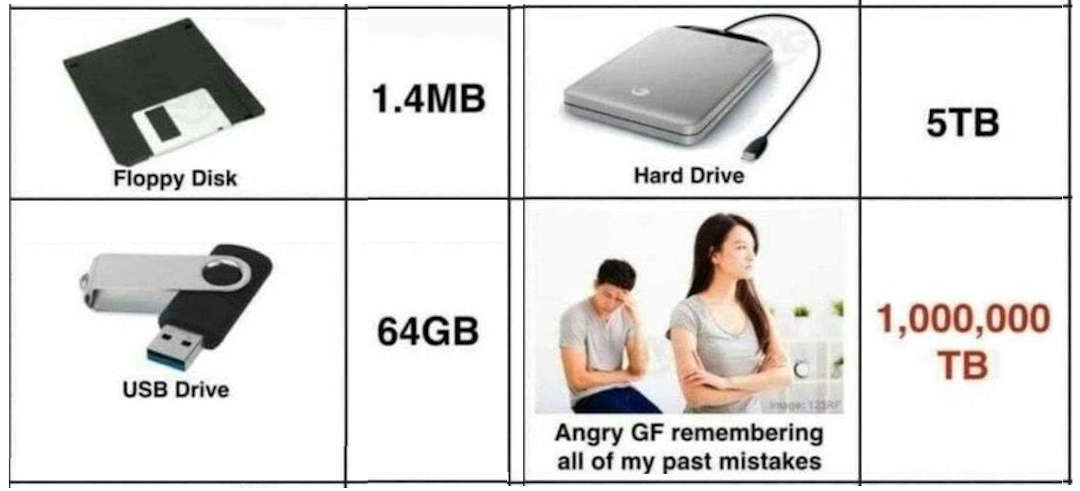
\includegraphics[width=0.90\linewidth]{os-Storage-HackingArticles}
\caption{Source: \url{https://linktr.ee/hackingarticles}}
\end{figure}
\end{frame}

% XXXXXXXXXXXXXXXXXXXXXXXXXXXXXXXXXXXXXXXXXXXXXXXXXXXXXXXXXXXXXXXXXXXXXXXXXX
\begin{frame}
\frametitle{Storage Failure Rates}
\begin{itemize}
\item MTTDL: Mean Time To Data Loss
\item MTTF: Mean Time To Failure
\item BackBlaze (Cloud Backup Services)
\end{itemize}
\begin{figure}
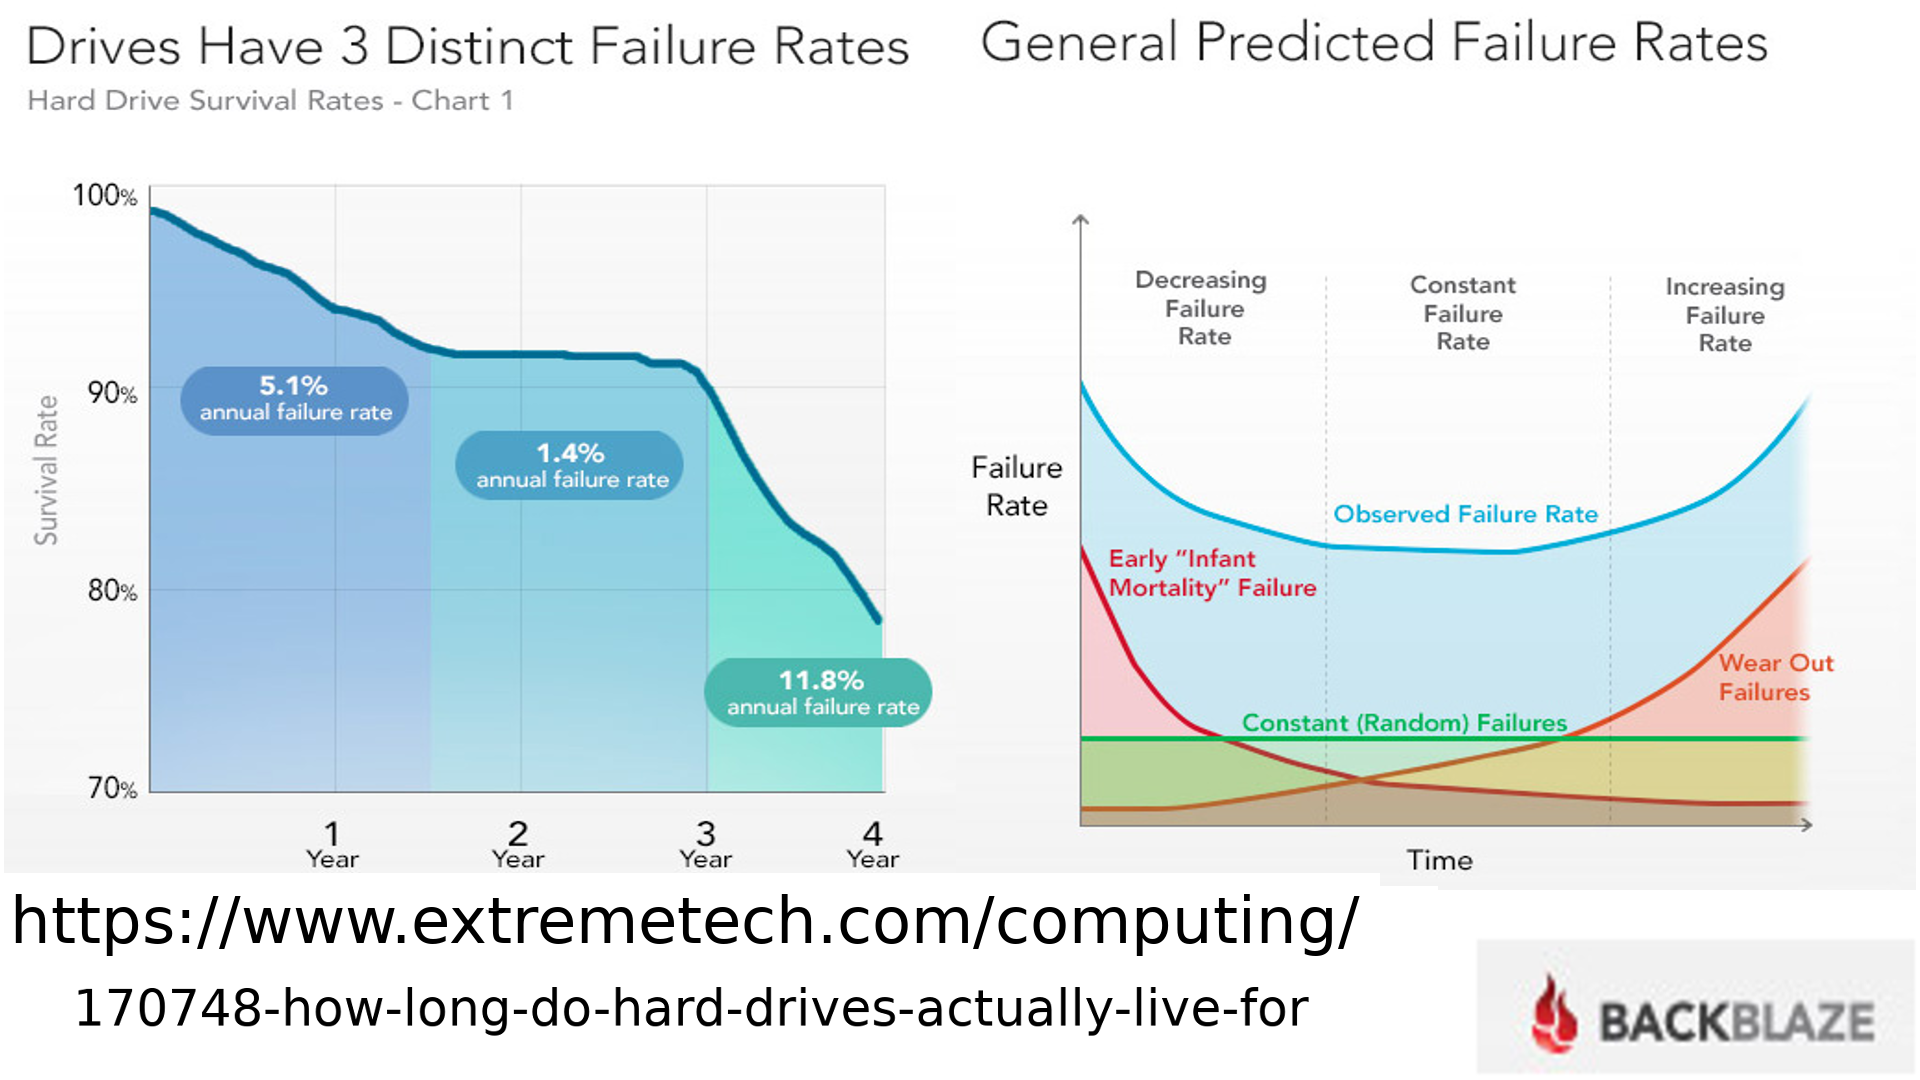
\includegraphics[width=0.60\linewidth]{os-extreme-tech}
\caption{BackBlaze --- Failure Rates of 25000 DISKS}
\end{figure}
\end{frame}

% XXXXXXXXXXXXXXXXXXXXXXXXXXXXXXXXXXXXXXXXXXXXXXXXXXXXXXXXXXXXXXXXXXXXXXXXXX
\section{Storage Management}
\begin{frame}
\frametitle{Storage Management}
\begin{itemize}
\item Attached-Storage.
\begin{itemize}
\item Host-Attached Storage: via I/O.
\item Network-Attached Storage (NAS): via distributed FileSystem.
\item Storage Area Network (SAN): dedicated Network.
\end{itemize}
\item Formating
\begin{itemize}
\item Low Level (Physical)
\item High Level (FileSystem)
\end{itemize}
\item Boot Block
\item Disk Partition
\begin{itemize}
\item ''MBR''-scheme
\begin{itemize}
\item upto 4 primary partition
\item upto 2 TB disk
\end{itemize}
\item ''GPT''-scheme
\begin{itemize}
\item ''unlimited'' partition
\item ''unlimited'' disk
\item redundancy
\end{itemize}
\end{itemize}
\item Swap Space Management: On Partition or FileSystem?
\end{itemize}
\end{frame}

% XXXXXXXXXXXXXXXXXXXXXXXXXXXXXXXXXXXXXXXXXXXXXXXXXXXXXXXXXXXXXXXXXXXXXXXXXX
\section{RAID}
\begin{frame}
\frametitle{RAID: Redundant Array of In* Disks}
\begin{itemize}
\item RAID 0, 1, 5, 6, 10, 100
\item Note (\url{http://www.commodore.ca/windows/raid5/raid5.htm}):
\begin{itemize}
\item RAID was created to enhance data performance, reliability and availability.
\item Striping, parity checking and mirroring are three primary functions of
      RAID systems.
\item RAID performs its functions transparent to the operating system.
\item Systems are typically defined by ranks consisting of five disks each
      connected to one or two Disk Array Controllers.
\item Different RAID levels provide varying degrees of speed and data protection.
\end{itemize}
\item Problems with RAID
\item Stable-Storage Implementation
\end{itemize}
\end{frame}

% XXXXXXXXXXXXXXXXXXXXXXXXXXXXXXXXXXXXXXXXXXXXXXXXXXXXXXXXXXXXXXXXXXXXXXXXXX
\begin{frame}
\frametitle{BIOS, Boot, \& Systemd}
\begin{itemize}
\item Firmware
\begin{itemize}
\item BIOS: Basic Input Output System.
\item UEFI: Unified Extensible Firmware Interface.
\item ACPI: Advanced Configuration and Power Interface.
\end{itemize}
\item Operating System (Boot) Loader
\begin{itemize}
\item BOOTMGT: Windows Bootmanager / Bootloader.
\item LILO:  Linux Loader.
\item GRUB:  GRand Unified Bootloader.
\end{itemize}
\item Operating System Initialization
\begin{itemize}
\item Init (legacy)
\item UpStart
\item Systemd
\end{itemize}
\end{itemize}
\end{frame}

% 8 XXXXXXXXXXXXXXXXXXXXXXXXXXXXXXXXXXXXXXXXXXXXXXXXXXXXXXXXXXXXXXXXXXXXXXXX
\section{Legacy BIOS}
\begin{frame}
\frametitle{Legacy BIOS}
\begin{itemize}
\item Check Settings.
\item Initialize CPU \& RAM.
\item POST: Power-On Self-Test.
\item Initialize ports, LANS, etc.
\item Load a Boot Loader.
\item Handover to the Boot Loader.
\item Provides "Native" (obsolete) Drivers only (not loadable).
\item Provides "INT" services .
\item Limitation.
\begin{itemize}
\item Technology of 1970s.
\item 16 bits software.
\item 20 bits address space (1 MB).
\item 31 bits disk space (2 TB).
\end{itemize}
\end{itemize}


\end{frame}

% XXXXXXXXXXXXXXXXXXXXXXXXXXXXXXXXXXXXXXXXXXXXXXXXXXXXXXXXXXXXXXXXXXXXXXXXXX
\begin{frame}
\frametitle{BIOS}
\begin{figure}
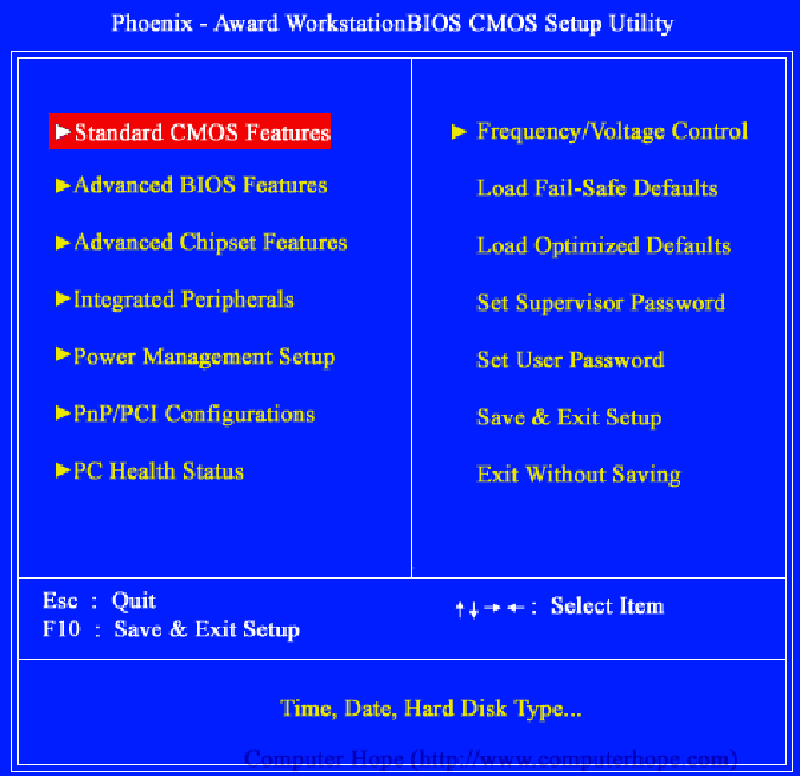
\includegraphics[width=0.45\linewidth]{os03-BIOS}
\caption{BIOS}
\end{figure}
\end{frame}

% XXXXXXXXXXXXXXXXXXXXXXXXXXXXXXXXXXXXXXXXXXXXXXXXXXXXXXXXXXXXXXXXXXXXXXXXXX
\section{UEFI}
\begin{frame}
\frametitle{UEFI}
\begin{itemize}
\item A Firmware Specification, not an Implementation!
\item No (INT) service after boot.
\item HII: Human Interface Infrastructure.
\item Protected Mode.
\item Flexible.
\begin{itemize}
\item Technology of 2000s.
\item writen in C.
\item (third party) loadable drivers and tools.
\item Emulate Legacy BIOS transition (MBR block, INT service).
\item UEFI Shell: environment shell for diagnostic (no need for DOS).
\end{itemize}
\item Problems
\begin{itemize}
\item Who controls the Hardware?
\item Is ''Secure Boot'' a good thing?
\item How about a \textbf{NASTY/LOCKING/TROJAN} UEFI implementation?
\item Different \textbf{DRIVERS}.
\end{itemize}
\end{itemize}
\end{frame}


% XXXXXXXXXXXXXXXXXXXXXXXXXXXXXXXXXXXXXXXXXXXXXXXXXXXXXXXXXXXXXXXXXXXXXXXXXX
\begin{frame}
\frametitle{UEFI}
\begin{figure}
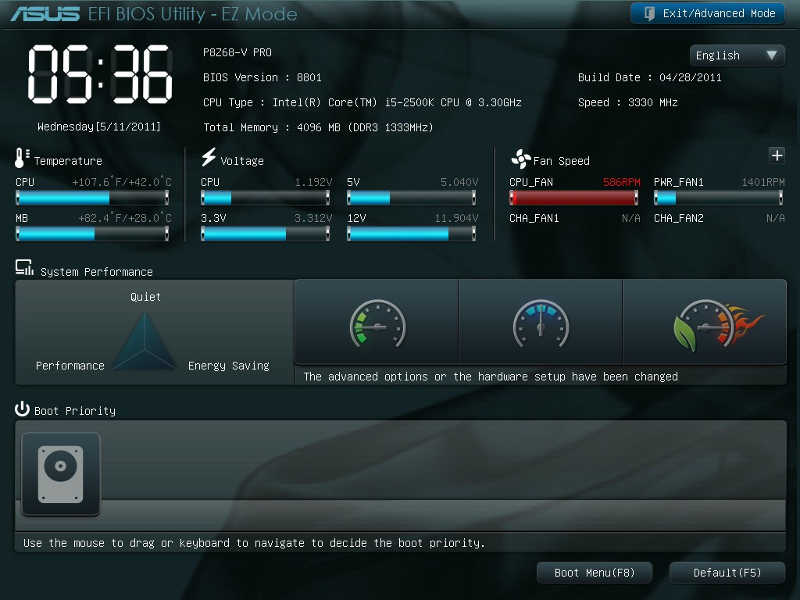
\includegraphics[width=0.59\linewidth]{os03-UEFI.jpg}
\caption{UEFI}
\end{figure}
\end{frame}

% XXXXXXXXXXXXXXXXXXXXXXXXXXXXXXXXXXXXXXXXXXXXXXXXXXXXXXXXXXXXXXXXXXXXXXXXXX
\begin{frame}
\frametitle{UEFI Boot}
\begin{figure}
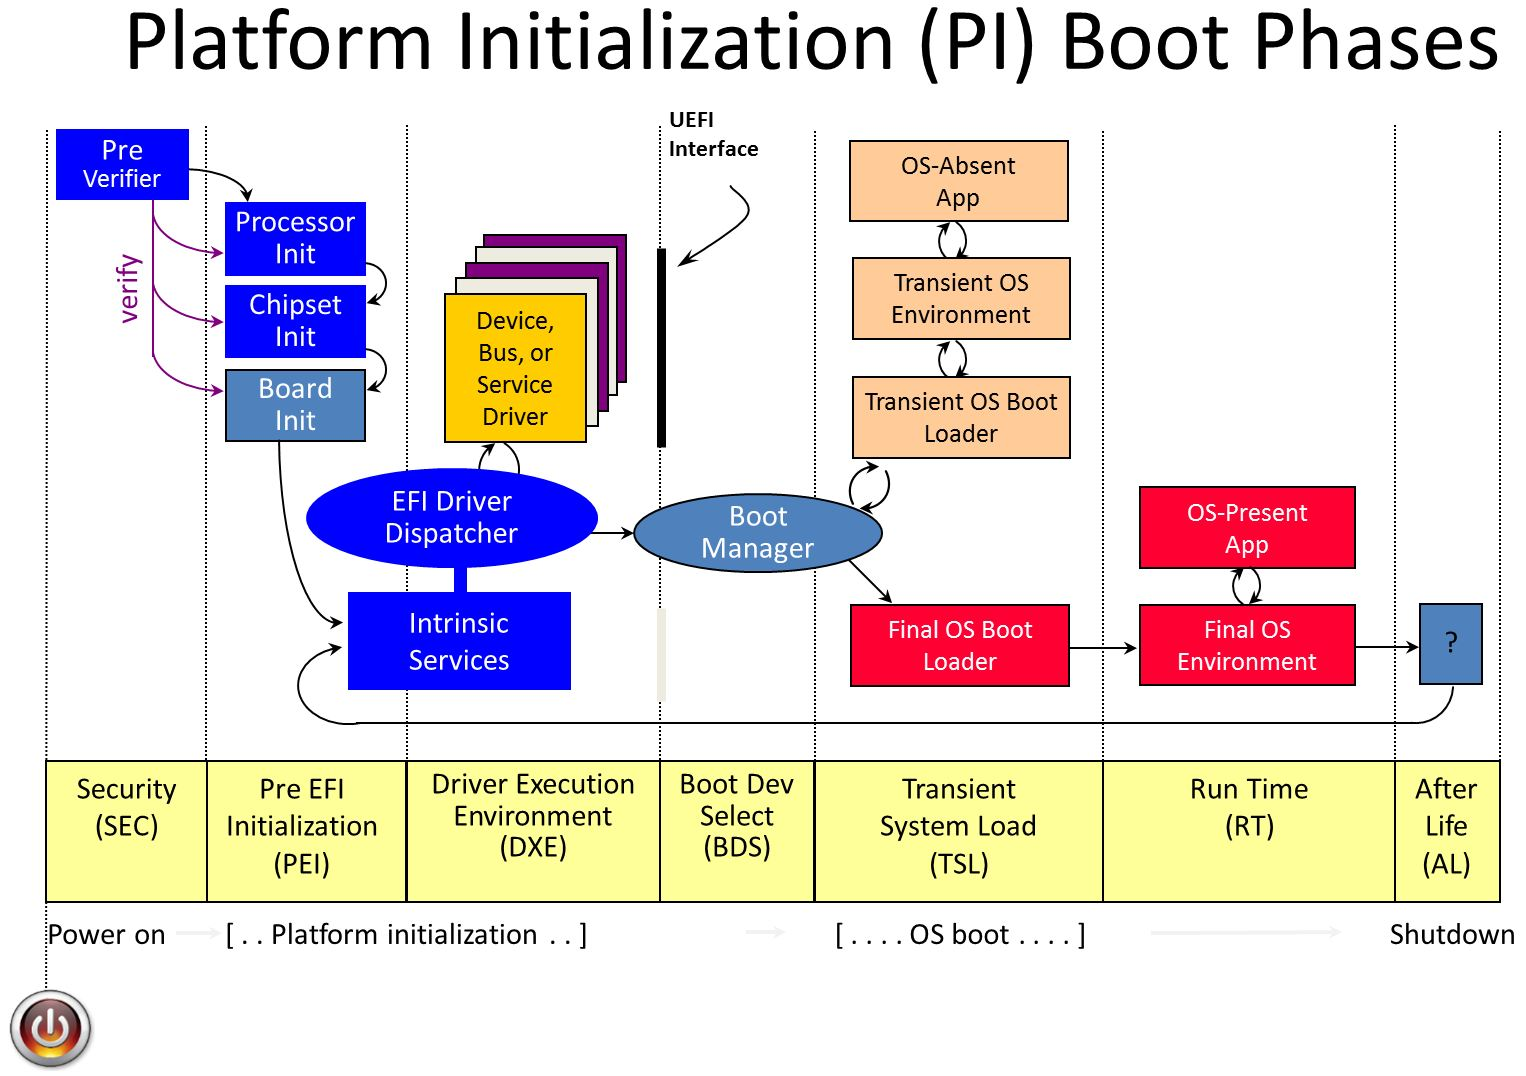
\includegraphics[width=0.51\linewidth]{os03-Jarlstrom-2014-PI-Boot-Phases-tianocore-org}
\caption{UEFI Boot Process\footnote{
Source Jarslstrom - 2014 - www.tianocore.org}.}
\end{figure}
\end{frame}

% XXXXXXXXXXXXXXXXXXXXXXXXXXXXXXXXXXXXXXXXXXXXXXXXXXXXXXXXXXXXXXXXXXXXXXXXXX
\section{Operating System (Boot) Loader}
\begin{frame}
\frametitle{Operating System (Boot) Loader}
\begin{itemize}
\item General
\begin{itemize}
\item How/Where to start the operating system?
\item What to do?
\item How many ways to boot?
\item How many types of OS?
\end{itemize}
\item Disk Partition
\begin{itemize}
\item MBR: Master Boot Record (1983).
\item GPT: GUID (Globally Unique Identifiers) Partition Table (2010s).
\end{itemize}
\item GRUB: GRand Unified Boot system
\begin{itemize}
\item Stage 1: a small boot.img inside the MBR.
\item Stage 1.5 (core.img): FileSystem drivers after MBR.
\item Stage 2: Kernel Selection: Windows, Linux, BSD, etc. 
\end{itemize}
\item GRUB2
\begin{itemize}
\item More flexible than GRUB legacy.
\item More automated than GRUB legacy.
\item Accept MBR and GPT.
\item Stage 1.5 (core.img): generated from diskboot.img.
\item No 1024 cylinder restriction.
\end{itemize}
\end{itemize}
\end{frame}

% XXXXXXXXXXXXXXXXXXXXXXXXXXXXXXXXXXXXXXXXXXXXXXXXXXXXXXXXXXXXXXXXXXXXXXXXXX
\section{GRUB Map}
\begin{frame}
\frametitle{GRUB Map}
\begin{figure}
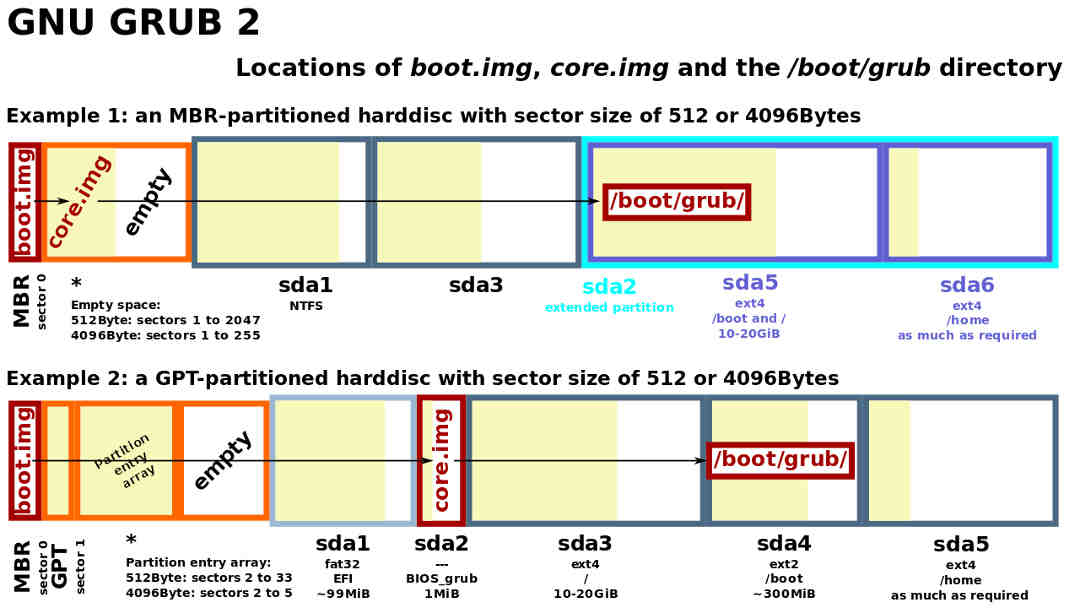
\includegraphics[width=0.69\linewidth]{os03-Shmuel-Csaba-Otto-Traian-2013-GRUB.jpg}
\caption{GRUB\footnote{Source Shmuel Csaba Otto Traian 2013}.}
\end{figure}
\end{frame}

% XXXXXXXXXXXXXXXXXXXXXXXXXXXXXXXXXXXXXXXXXXXXXXXXXXXXXXXXXXXXXXXXXXXXXXXXXX
\section{init (SYSV legacy)}
\begin{frame}
\frametitle{init (SYSV legacy)}
\begin{itemize}
\item File: \texttt{/etc/inittab}.
\item Folders: \texttt{/etc/rcX.d} --- X = runlevel.
\begin{itemize}
\item Seven (7) different runlevels: 
\begin{itemize}
\item 0 (shutdown).
\item 1 (single-user/admin).
\item 2 (multi-user non net).
\item 3 (standard).
\item 4 (N/A).
\item 5 (3+GUI).
\item 6 (reboot).
\end{itemize}
\item SXX-YYY: Start
\item KXX-YYY: Kill.
\end{itemize}
\item One script at a time in order.
\item dependency is set manually.
\end{itemize}
\end{frame}

% XXXXXXXXXXXXXXXXXXXXXXXXXXXXXXXXXXXXXXXXXXXXXXXXXXXXXXXXXXXXXXXXXXXXXXXXXX
\section{UpStart - Ubuntu}
\begin{frame}
\frametitle{UpStart - Ubuntu}
\begin{itemize}
\item Developer: Ubuntu.
\item Folder: \texttt{/etc/init/}.
\item Control: \texttt{initctl}.
\begin{itemize}
\item \texttt{initctl list} -- listing all processes managed by upstart.
\end{itemize}
\item better support for hotplug devices.
\item cleaner service management.
\item faster service management.
\item asynchronous.
\end{itemize}
\end{frame}

% XXXXXXXXXXXXXXXXXXXXXXXXXXXXXXXXXXXXXXXXXXXXXXXXXXXXXXXXXXXXXXXXXXXXXXXXXX
\section{The All New "systemd"}
\begin{frame}
\frametitle{The All New "systemd"}
\begin{itemize}
\item Replaces (SYSV) init and UpStart.
\begin{itemize}
\item better concurency handling: Faster!
\item better dependencies handling: No more "S(tarts)" and "K(ills)".
\item better crash handling: automatic restart option.
\item better security: group protection from anyone including superusers.
\item simpler config files: reliable and clean scripts.
\item hotplug: dynamic start/stop.
\item supports legacy systems (init).
\item overhead reducing.
\item unified management way for all distros.
\item bloated: doing more with more resources.
\item linux specific: NOT portable.
\end{itemize}
\end{itemize}
\end{frame}

% XXXXXXXXXXXXXXXXXXXXXXXXXXXXXXXXXXXXXXXXXXXXXXXXXXXXXXXXXXXXXXXXXXXXXXXXXX
\section{systemctl}
\begin{frame}[fragile]
\frametitle{systemctl 01}
\begin{lstlisting}[basicstyle=\ttfamily\small]
for II in      \
   'systemctl list-unit-files | head -8; echo "(...)";
       systemctl list-unit-files| tail -8' \
   'systemd-analyze blame | wc -l; echo "===";
       systemd-analyze blame | head -15' \
   'systemctl --full  | wc -l; echo "===";
       systemctl --full  | head -10' \
   'systemctl list-units  | wc -l; echo "===";
       systemctl list-units  | head -10' \
   'systemctl list-units |grep .service|wc -l;echo "===";
       systemctl list-units|grep .service|head -10' \
   'systemctl list-units  | grep ssh.service' \
   'systemctl status ssh.service' \
   'systemctl is-enabled ssh' \
   'journalctl' \
   'journalctl -b' \
do
...
\end{lstlisting}

\end{frame}

% XXXXXXXXXXXXXXXXXXXXXXXXXXXXXXXXXXXXXXXXXXXXXXXXXXXXXXXXXXXXXXXXXXXXXXXXXX
\begin{frame}[fragile]
\frametitle{systemctl 02}
\begin{figure}
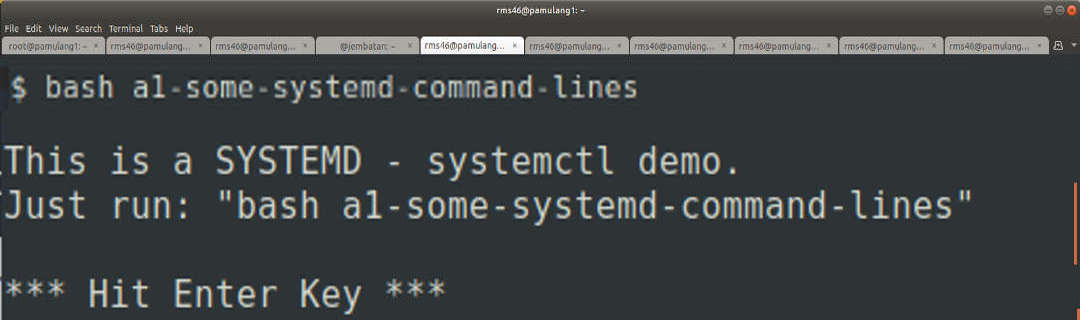
\includegraphics[width=.93\linewidth]{os-systemd01.jpg}
\caption{bash a1-some-systemd-command-lines}
\end{figure}
\end{frame}

% XXXXXXXXXXXXXXXXXXXXXXXXXXXXXXXXXXXXXXXXXXXXXXXXXXXXXXXXXXXXXXXXXXXXXXXXXX
\begin{frame}[fragile]
\frametitle{systemctl 03}
\begin{figure}
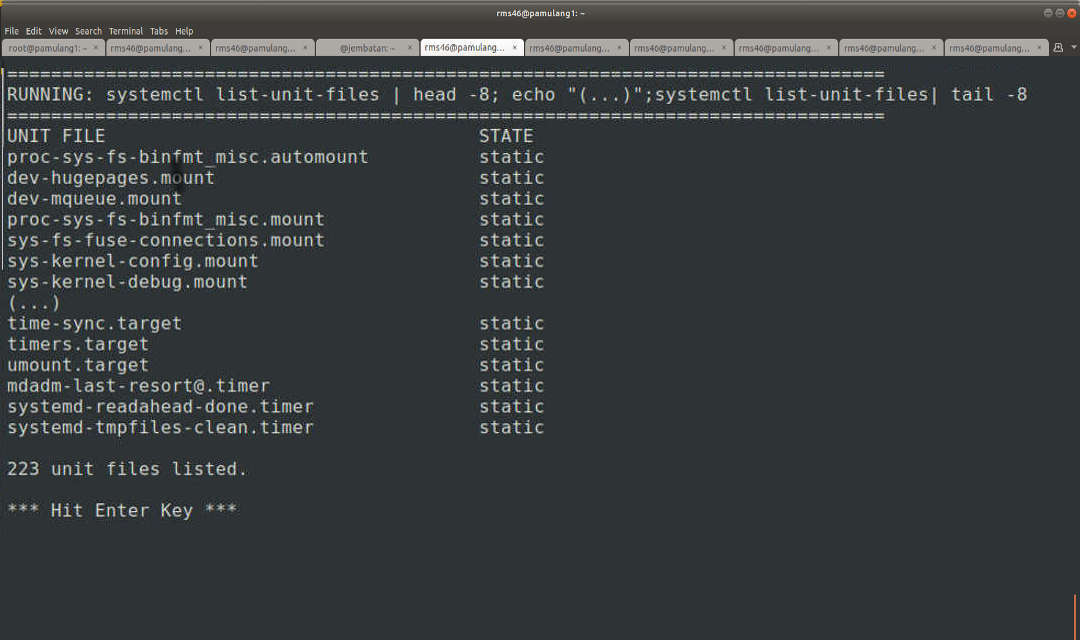
\includegraphics[width=.74\linewidth]{os-systemd02.jpg}
\caption{systemctl list-unit-files}
\end{figure}
\end{frame}

% XXXXXXXXXXXXXXXXXXXXXXXXXXXXXXXXXXXXXXXXXXXXXXXXXXXXXXXXXXXXXXXXXXXXXXXXXX
\begin{frame}[fragile]
\frametitle{systemctl 04}
\begin{figure}
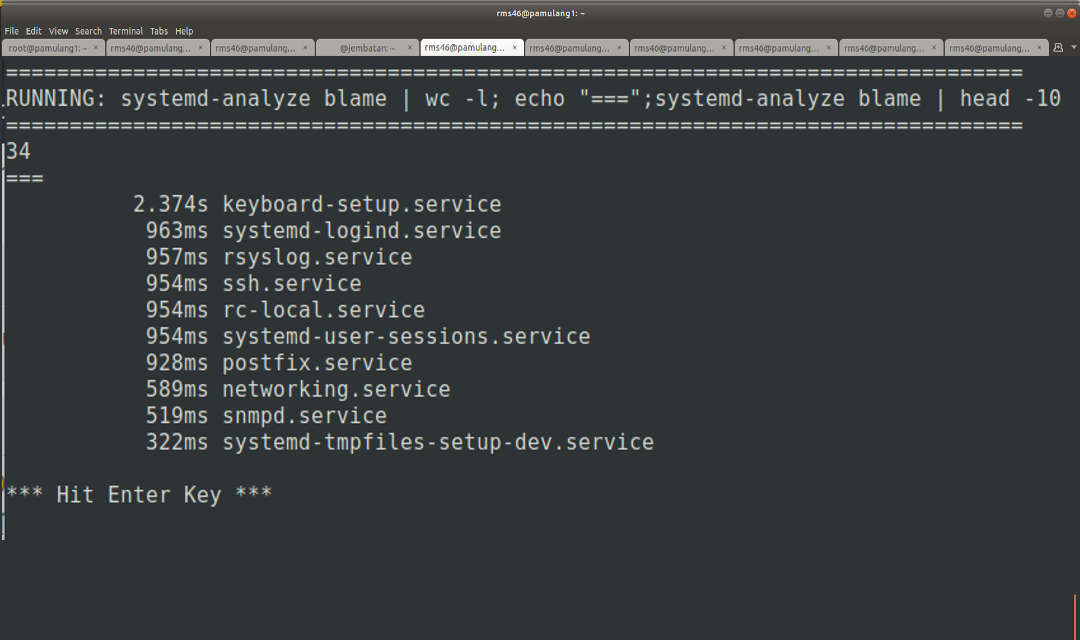
\includegraphics[width=.74\linewidth]{os-systemd03.jpg}
\caption{systemd-analyze blame}
\end{figure}
\end{frame}

% XXXXXXXXXXXXXXXXXXXXXXXXXXXXXXXXXXXXXXXXXXXXXXXXXXXXXXXXXXXXXXXXXXXXXXXXXX
\begin{frame}[fragile]
\frametitle{systemctl 05}
\begin{figure}
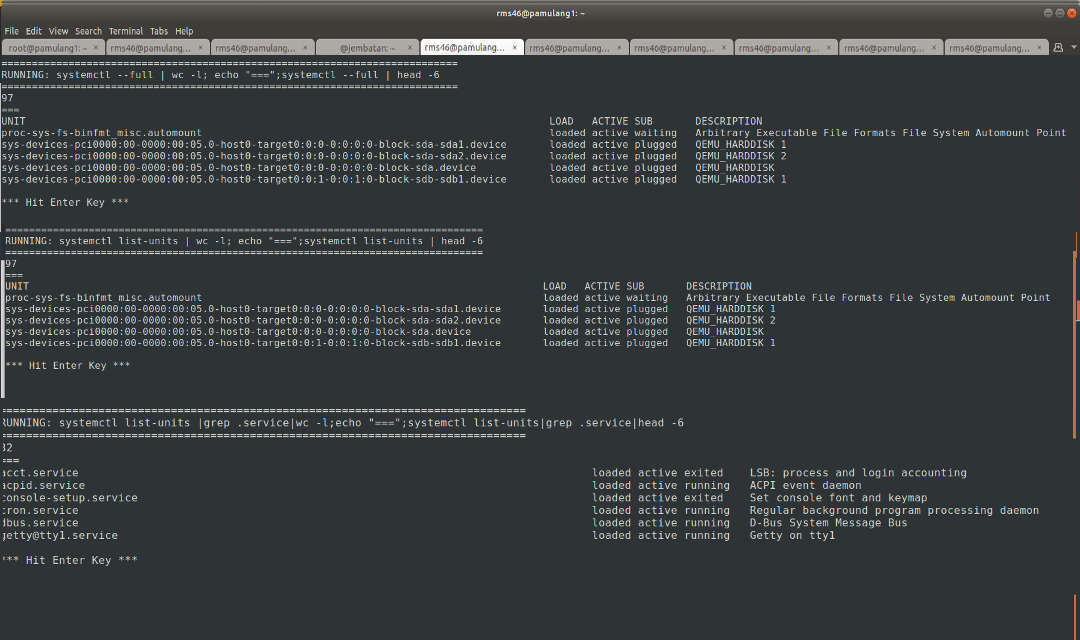
\includegraphics[width=.74\linewidth]{os-systemd04.jpg}
\caption{systemctl --full; systemctl list-units}
\end{figure}
\end{frame}

% XXXXXXXXXXXXXXXXXXXXXXXXXXXXXXXXXXXXXXXXXXXXXXXXXXXXXXXXXXXXXXXXXXXXXXXXXX
\begin{frame}[fragile]
\frametitle{systemctl 06}
\begin{figure}
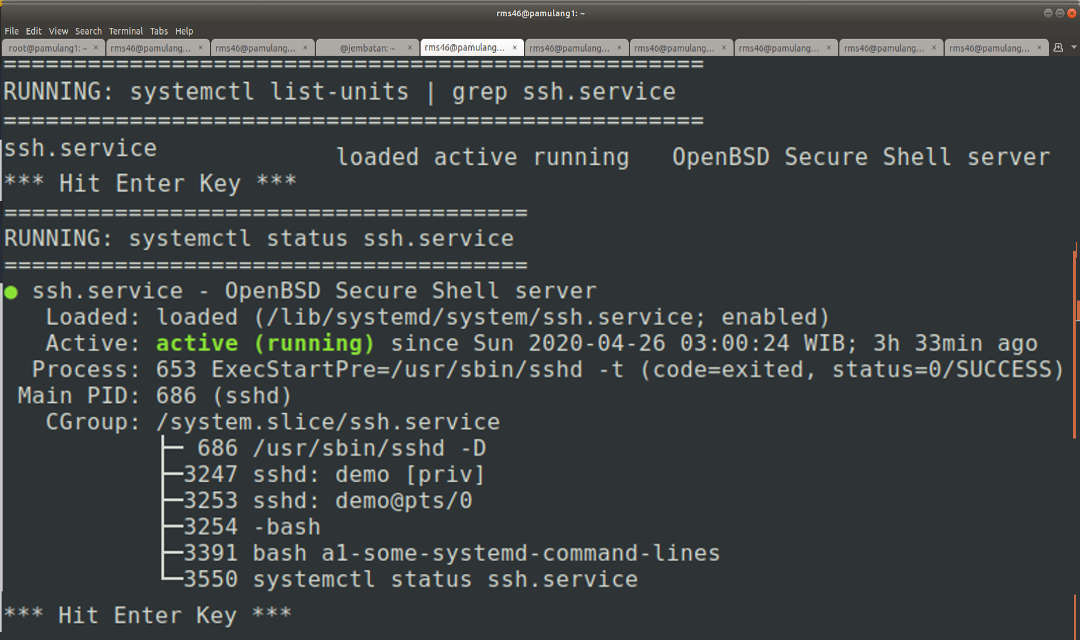
\includegraphics[width=.74\linewidth]{os-systemd05.jpg}
\caption{systemctl status ssh.service}
\end{figure}
\end{frame}

% XXXXXXXXXXXXXXXXXXXXXXXXXXXXXXXXXXXXXXXXXXXXXXXXXXXXXXXXXXXXXXXXXXXXXXXXXX
\begin{frame}[fragile]
\frametitle{systemctl 07}
\begin{figure}
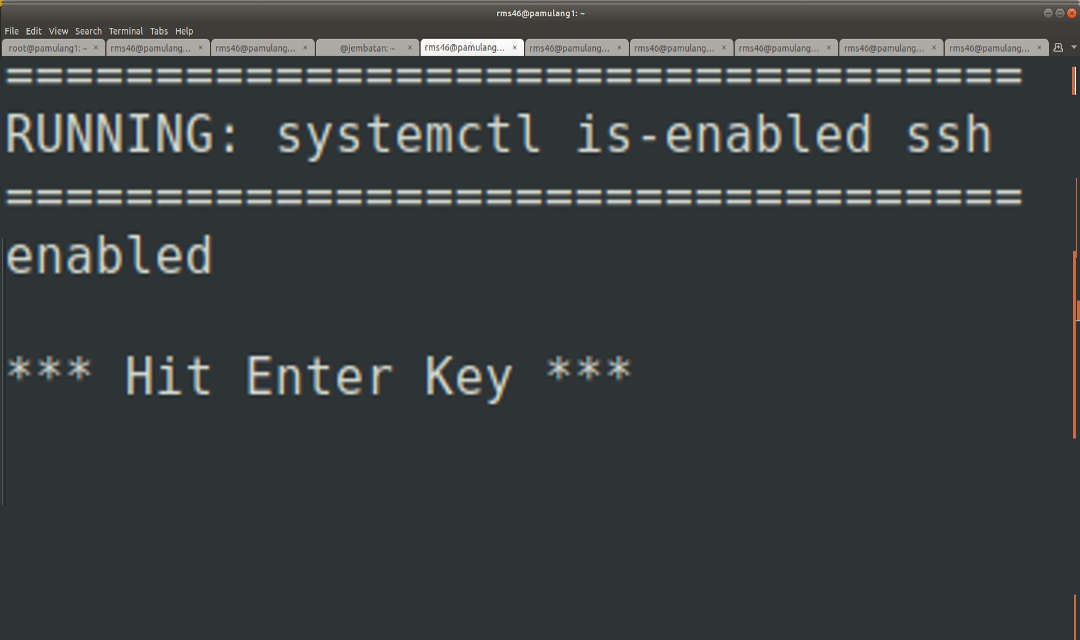
\includegraphics[width=.74\linewidth]{os-systemd06.jpg}
\caption{systemctl is-enabled ssh}
\end{figure}
\begin{table}
\end{table}
\end{frame}

% XXXXXXXXXXXXXXXXXXXXXXXXXXXXXXXXXXXXXXXXXXXXXXXXXXXXXXXXXXXXXXXXXXXXXXXXXX
\end{document}

